\documentclass{standalone}
\usepackage{tikz}
\usepackage{array}

\begin{document}

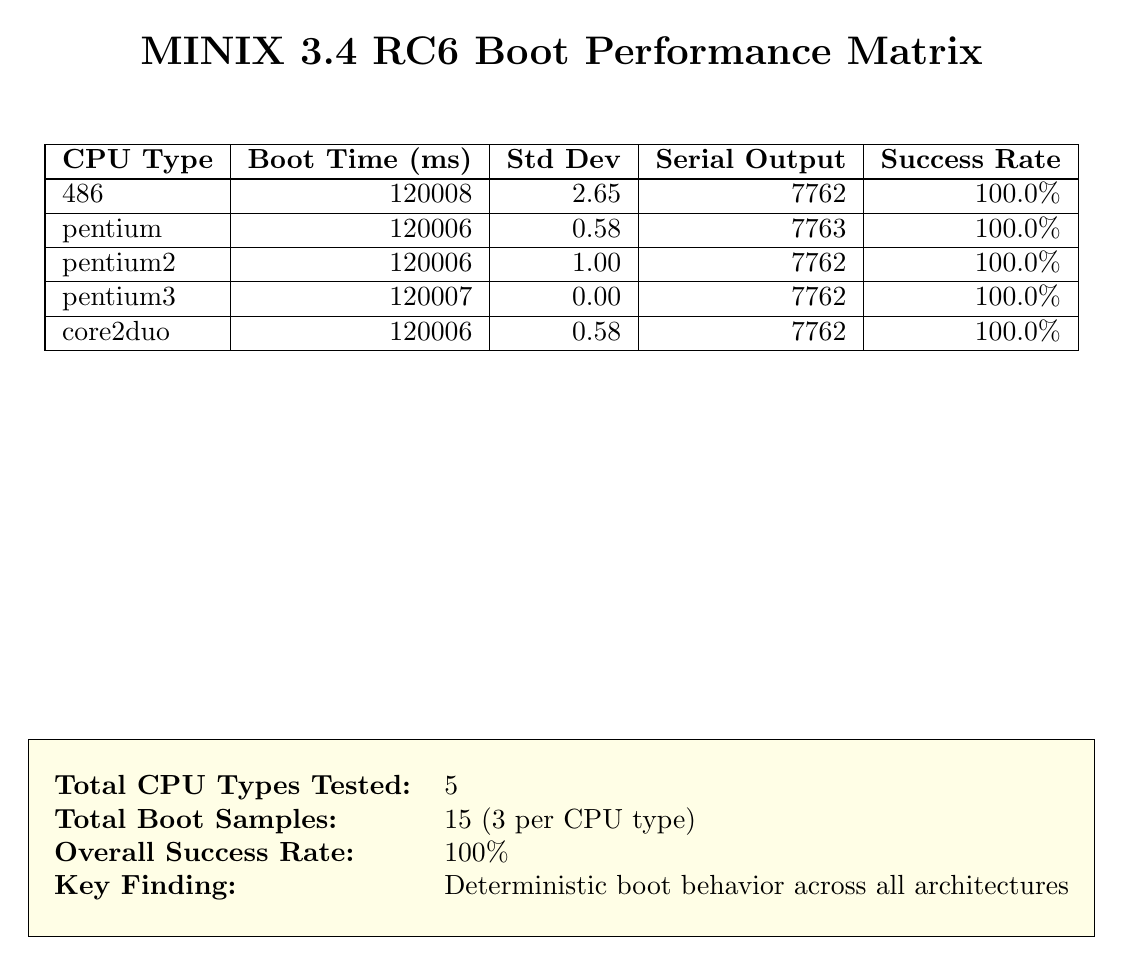
\begin{tikzpicture}

% Title
\node[font=\Large\bfseries] at (0, 12) {MINIX 3.4 RC6 Boot Performance Matrix};

% Table
\node at (0, 9.5) {
\begin{tabular}{|l|r|r|r|r|}
\hline
\textbf{CPU Type} & \textbf{Boot Time (ms)} & \textbf{Std Dev} & \textbf{Serial Output} & \textbf{Success Rate} \\
\hline
486 & 120008 & 2.65 & 7762 & 100.0\% \\
\hline
pentium & 120006 & 0.58 & 7763 & 100.0\% \\
\hline
pentium2 & 120006 & 1.00 & 7762 & 100.0\% \\
\hline
pentium3 & 120007 & 0.00 & 7762 & 100.0\% \\
\hline
core2duo & 120006 & 0.58 & 7762 & 100.0\% \\
\hline

\end{tabular}
};

% Summary section
\node[draw=black, fill=yellow!10, minimum width=8cm, minimum height=2.5cm] at (0, 2) {
\begin{tabular}{ll}
\textbf{Total CPU Types Tested:} & 5 \\
\textbf{Total Boot Samples:} & 15 (3 per CPU type) \\
\textbf{Overall Success Rate:} & 100\% \\
\textbf{Key Finding:} & Deterministic boot behavior across all architectures
\end{tabular}
};

\end{tikzpicture}

\end{document}